\section{Method}

Our framework introduces a novel guidance strategy built upon a frozen SDXL backbone, complemented by a lightweight, trainable Resampler network. An overview of the full architecture is provided in Figure~\ref{fig:guidance}. The core of our method consists of two inference-time modules: \textbf{Relative Self-Attention Guidance (RSAG)} for structural preservation and \textbf{Style-Aligned Sparse Attention} for controllable stylization. While the guidance modules themselves are tuning-free, they leverage style features extracted by a lightweight, trainable Resampler network that maps outputs from a frozen CLIP image encoder into the diffusion model's feature space.

\begin{figure*}[t]
\centering
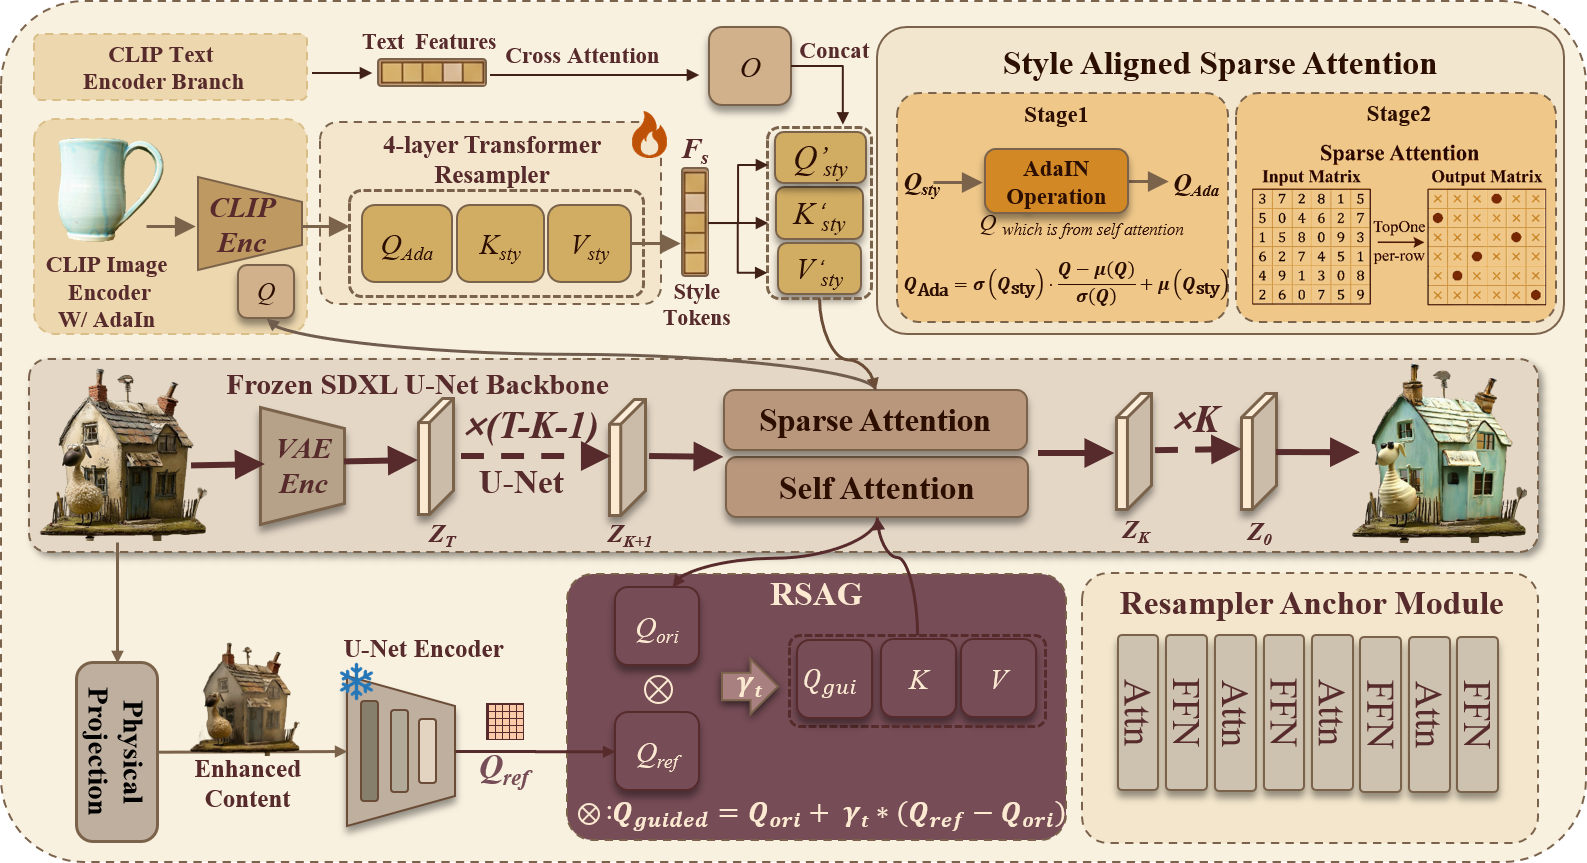
\includegraphics[width=1.0\textwidth]{images/2mechnism.png}
\caption{Overview of the Rationale framework. The center pipeline shows the SDXL denoising process: the content image is VAE-encoded into a noisy latent $Z_T$, progressively denoised through U-Net blocks, and decoded to the output image. Two modules act jointly at each U-Net block. \textbf{(A) Style-Aligned Sparse Attention:} The style image is encoded by the frozen CLIP encoder; the spatial query $Q_\text{ori}$ from the U-Net is modulated via AdaIN using global style statistics and fed into the trainable Resampler alongside CLIP keys/values, producing structure-aligned style tokens injected via Top-1 sparse attention. \textbf{(B) RSAG:} The content image passes through the Physical Projection module to produce an enhanced structural prior; self-attention queries are cached from a frozen U-Net pass and used at each denoising step to steer generation via $Q_\text{guided} = Q_\text{ori} + \gamma_t(Q_\text{ref} - Q_\text{ori})$. The Resampler is the only trainable component.}
\label{fig:guidance}
\end{figure*}

\subsection{Relative Self-Attention Guidance (RSAG)}

Inspired by classifier-free guidance, which steers the generation process by taking a step in the direction of the score difference field, we frame our structural guidance problem from a distributional perspective. Let the self-attention queries at a original latent and those from a reference latent be sampled from two local distributions, $q_\text{ori}$ and $q_\text{ref}$, respectively. The optimal direction to shift $Q_\text{ori}$ toward $Q_\text{ref}$ can be seen as a step along the score difference, $u^*(Q) = \nabla_Q \log P(Q_\text{{ref}}) - \nabla_Q \log P(Q_\text{ori})$.

While directly computing this score difference $u^*$ is intractable, we can form a practical approximation. Assuming the score functions are locally smooth, the difference can be approximated by a first-order Taylor expansion around $Q_\text{ori}$:
\begin{equation}
    u^*(Q) = \nabla_Q \log P(Q_\text{ref}) - \nabla_Q \log P(Q_\text{ori}) \approx \mathbf{H}(Q_\text{ori}) (Q_\text{ref} - Q_\text{ori}),
    \label{eq:taylor_approx}
\end{equation}
where $\mathbf{H}(Q_\text{ori})$ is a matrix related to the Hessian of the log-densities. This reveals that the optimal guidance direction is, to a first order, proportional to the simple difference vector $(Q_\text{ref} - Q_\text{ori})$.
Based on this insight, we adopt a practical and efficient heuristic by simplifying the matrix $\mathbf{H}(Q_\text{ori})$ to a time-dependent scalar $\gamma_t$. This leads to our guidance formulation (a detailed regret bound analysis in Appendix ):
\begin{equation}
    Q_\text{guided} = Q_\text{ori} + \gamma_t (Q_\text{ref} - Q_\text{ori}),
    \label{eq:rsag_update}
\end{equation}
where $Q_\text{guided}$ is the guided query. The coefficient $\gamma_t$ follows a cosine schedule, $\gamma_t = (1 - \cos(\pi t / T))/2$, where $t$ is the current timestep counted \emph{downward} from $T$ (fully noisy) to $0$ (clean), so $\gamma_T = 1$ at the start and $\gamma_0 = 0$ at the end. This schedule aligns with the signal-to-noise ratio progression in diffusion models: structural alignment is applied most strongly during the early, high-noise stages where global layout is determined, and relaxed in the later low-noise stages to allow fine detail refinement. The guided query then replaces the original in the self-attention computation:
\begin{equation}
    A_t^{(l)} = \text{Softmax}\!\left(\frac{Q_\text{guided} (K_\text{ori})^\top}{\sqrt{d}}\right) V_\text{ori},
\end{equation}
where $K_\text{ori}$ and $V_\text{ori}$ are the original keys and values derived from the frozen SDXL self-attention layers, $d$ is the dimension of the attention head, and $A_t^{(l)}$ is the updated attention output for layer $l$. This modification is localized to query computation, preserving the architectural integrity of the pretrained SDXL attention mechanism. The construction of the reference queries $Q_\text{ref}$ is detailed below.

\paragraph{Reference Query Construction.}
To clarify how the reference queries $Q_\text{ref}$ are obtained, we introduce a one-time pre-computation step. First, a reference image is generated by applying our custom-implemented lightweight structural and illumination enhancement modules (see Appendix for detailed algorithms and source code) to the original content image. Specifically, these modules leverage deterministic edge extraction operators (e.g., Canny) to derive geometric priors and simulate environment lighting to synthesize shading variations, avoiding the need for complex 3D reasoning. This Enhancement Module serves as a Structural Anchor, extracting salient edges and depth cues to guide the attention toward geometric structure rather than pixel noise. This enhanced image serves as the structural prior. We then perform a complete denoising trajectory (25 DDIM steps, consistent with inference) through the frozen SDXL U-Net using this reference image and a neutral text prompt (e.g., ``a high-quality photograph"). During this trajectory, we cache the self-attention query vectors from all relevant attention blocks across all timesteps. These cached vectors become the reference queries, $Q_\text{ref}^{(l,t)}$, providing a stable, layer- and time-specific structural target for the main generation process. This caching strategy ensures that the RSAG module itself operates efficiently at inference time without any parameter updates.

\subsection{Style Injection via Style-Aligned Sparse Attention}

Unlike prior adapter-based methods that inject style via keys or values indiscriminately, this work modulates query statistics to control \textit{where} attention is paid rather than just \textit{what} features are aggregated, yielding finer spatial control. We achieve this by introducing a structure-aware pre-modulation step before the style features are even extracted.

The process begins by utilizing the frozen \textbf{CLIP Image Encoder} to extract raw patch embeddings from the style image ($I_s$). Let these serve as the foundational style keys and values, denoted as $K_{\text{sty}}$ and $V_{\text{sty}}$. Concurrently, we extract a spatial query $Q$ from the U-Net's self-attention branch. This spatial $Q$ inherently captures the geometric structure and layout of the current generation step. 

Before querying the style information, we modulate this spatial query $Q \in \mathbb{R}^{N \times d}$ (where $N$ is the spatial sequence length and $d$ is the feature dimension) with a base style query $Q_{\text{sty}} \in \mathbb{R}^{1 \times d}$ (derived from the global CLIP embedding) using \textbf{Adaptive Instance Normalization (AdaIN)}~\cite{huang2017arbitrary}:
\begin{equation}
    Q_{\text{Ada}} = \sigma(Q_{\text{sty}})\cdot \frac{Q - \mu(Q)}{\sigma(Q)} + \mu(Q_{\text{sty}}),
\end{equation}
where $\mu(\cdot)$ and $\sigma(\cdot)$ denote channel-wise mean and standard deviation. Specifically, the statistics for $Q$ are aggregated across the spatial dimension $N$, yielding $\mu(Q), \sigma(Q) \in \mathbb{R}^{1 \times d}$, while the statistics for the 1D global style token $Q_{\text{sty}}$ are its own channel values. Applying AdaIN at this stage aligns the structural query to the global style statistics through channel-wise broadcasting, ensuring dimension compatibility. Crucially, we apply AdaIN strictly to the spatial queries ($Q$), leaving the CLIP-extracted keys and values ($K_{\text{sty}}, V_{\text{sty}}$) untouched. Because these keys and values already encode the pure target style, modulating them disrupts their intrinsic semantic integrity. Our empirical tests confirm this: attempting to modulate the keys or values severely degrades both structural layout and style fidelity.

The structurally-anchored query $Q_{\text{Ada}}$, along with $K_{\text{sty}}$ and $V_{\text{sty}}$, is then fed into our lightweight \textbf{Resampler}—a 4-layer transformer with 8 attention heads per layer—designed to capture high-fidelity style representations without the artifacts typical of simple linear projectors. Inside the Resampler, cross-attention is performed, allowing the spatially-aware $Q_{\text{Ada}}$ to selectively aggregate relevant stylistic details from the CLIP patches. The Resampler processes this into a fixed set of compact, structure-aligned style tokens $F_s$:
\begin{equation}
    F_s = \text{Resampler}(Q_{\text{Ada}}, K_{\text{sty}}, V_{\text{sty}}).
\end{equation}

These spatially-aware style tokens are then projected into the final style components $(Q'_{\text{sty}}, K'_{\text{sty}}, V'_{\text{sty}})$ for the main U-Net's cross-attention layers. To enforce a strict one-to-one correspondence and prevent style leakage across semantic regions, a deterministic sparse mask is applied during the main cross-attention computation:
\begin{equation}
    O_{\text{style}} = \text{Softmax}\!\left( \text{Top-1}\!\left(\frac{Q'_{\text{sty}}(K'_{\text{sty}})^{\!\top}}{\sqrt{d}}\right) \right)V'_{\text{sty}},
\end{equation}
where $\text{Top-1}(\cdot)$ retains only the maximum score per query, yielding deterministic sparsity. The final output combines the text- and style-conditioned responses through a linear blend:
\begin{equation}
    O' = O + \lambda_{s}O_{\text{style}},
\end{equation}
where $O$ is the original text-conditioned cross-attention output, and the parameter $\lambda_s \in [0, 1]$ controls the relative contribution of the style features.

\paragraph{Local Style Transfer.}
For spatially targeted stylization, we integrate a binary mask $M \in \{0,1\}^N$ into the sparse attention, modulating the attention scores before the Top-1 operation:
\begin{equation}
    A_\text{local} = \text{Top-1}\!\left(\frac{Q'_{\text{sty}}(K'_{\text{sty}})^{\!\top}}{\sqrt{d}} \odot M \right),
\end{equation}
where style tokens interact only with the masked spatial regions, ensuring zero style leakage into the background.

\subsection{Discussion and Implementation}

The RSAG module stabilizes the dynamics of self-attention through a fixed structural prior, while the Style-Aligned Sparse Attention mechanism modulates queries to inject style semantics. By synergizing these parameter-free guidance modules with a lightweight, trainable Resampler network, our framework achieves robust, structure-preserving stylization that balances performance with computational efficiency.

The trainable Resampler network is optimized on our self-curated SMSS dataset, which contains 60,000 images featuring a diverse and balanced range of styles and materials. We trained the network for 100,000 steps using the Adam optimizer with a fixed learning rate of 5e-5 and a batch size of 4, optimizing for the original SDXL denoising loss. All experiments were conducted on a single NVIDIA RTX 4090 GPU. At a 1024$\times$1024 resolution, excluding the one-time pre-computation caching step, our active guidance modules only introduce a 39\% increase in per-step generation time—a deliberate trade-off for improved structural consistency—due to the additional computations in the attention mechanism. The primary memory and computational overhead stems from the initial full denoising rollout required for caching multi-layer reference queries in the RSAG module (detailed computational cost analysis see Appendix).